\documentclass[12pt]{article}

% document class defines document-wide parameters. 
% You will probably use ``article'' for everything but posters and slides

% --- text and text block -----------------------

\usepackage[margin = 1in]{geometry} % controls page margins
\usepackage{setspace}               % controls line spacing

\usepackage{parskip}
% ``parskip'' is used to get (a) space between paragraphs and
% (b) no indentation at new paragraphs.
% This makes this particular document easier to read, 
% but I do NOT recommend using parskip ordinarily
% (except for problem sets maybe)

\usepackage{enumitem} % [nosep] option for lists
                     

% --- math things -----------------------

\usepackage{amsmath} % commonly used for enhanced math commands
\usepackage{amssymb} % commonly used for helpful symbols and fonts
                     % many people also load ``amsfonts''
                     % but amssymb loads amsfonts, so it's not necessary



% --- tables, figues, other floats -----------------------

\usepackage{float}    % float parameters

% graphics:
\usepackage{graphicx} % capabilites for inserting graphics
\usepackage{rotating} % if you want sideways graphics
\usepackage{subcaption} % if you want sub-figures
% \usepackage{placeins} 
%   ``placeins'' contains a helpful \FloatBarrier command
%   which prevents figures from bleeding across sections


% tables
\usepackage{booktabs} % commonly used to make tables prettier
\usepackage{dcolumn} % aligns table column text along a decimal pt
\usepackage{multirow} % cells spanning multi rows/cols



% --- other document logic/capabilities -----------------------

\usepackage{hyperref}            % hyperlinks
  \hypersetup{colorlinks = true, % link colors
              citecolor = black, 
              linkcolor = black, 
              urlcolor = teal}
\usepackage{xcolor}    % more colors (don't go too crazy)
\usepackage{todonotes} % print yourself to-do notes



% --- fancy code blocks -----------------------

% WARNING to workshop participants:
% These ``listings'' settings are included to make code blocks prettier,
%   but ``listings'' is inessential unless you want to make pretty code blocks,
%   which should be rare unless you're describing computer algorithms.
% I would NOT paste these settings into your future work.

% If you're interested in printing code, you might also check out ``minted''.
% Minted prints prettier code blocks, 
% but it depends on pygments (http://pygments.org/) which can be a pain

\usepackage{listings}

\definecolor{lgray}{gray}{0.925}

\lstset{ 
  backgroundcolor = \color{lgray},
  basicstyle = \ttfamily, % code style
  breakatwhitespace = true,      % if automatic break only happen at whitespace
  breaklines = false,            % automatic line breaking
  columns=fullflexible,          % kerning thing
  commentstyle = \color{gray},   % comment style
  escapeinside = {\% *}{*)},     % for using LaTeX within code
  keepspaces = true,             % keeps spaces for indentation 
                                 % (needs columns = flexible ?)
  language = TeX,                % the language of the code
  % morekeywords = {*,...},        % for adding more keywords
  showstringspaces = false      % underline spaces within strings only
}





\begin{document}

\title{{\LaTeX} Starter Guide}
\author{Michael DeCrescenzo%
          \thanks{Ph.D.\ Candidate, Political Science, University of Wisconsin--Madison. This handout borrows heavily past workshop materials created and passed down by Matthew Holleque, Sarah Niebler, and Dave Ohls, Sarah Bouchat, Nat Olin, Richard Loeza, and Jos\'e Luis Enr\'iquez Chi\~nas, and Michael Masterson.}}
\date{Updated \today}
\maketitle


\begin{abstract}
  This document describes and exemplifies many important {\LaTeX} concepts and best-practices. It discusses document setup, important commands and environments, text formatting, math, figures and tables, and so on. This document (a \lstinline{.pdf} file) is distributed alongside the source code used to create it (a \lstinline{.tex} file), allowing new {\LaTeX} users to see how {\LaTeX} code becomes printed content. The source code, along with other workshop materials, can be found on the workshop's Github page.%
    \footnote{\url{https://github.com/mikedecr/latex-workshop-2018}}
\end{abstract}

\tableofcontents

\section{How to read this document}

This document is intended to teach {\LaTeX} by example. The text contains a discussion of {\LaTeX} commands, but for instructional purposes it will also be valuable to download, inspect, and modify the source code%
  \footnote{I advise that you preserve an original copy of the source code, for future reference. The file can be copied from here: \url{https://raw.githubusercontent.com/mikedecr/latex-workshop-2018/master/handout/latex-handout-2018.tex}} yourself. 

Examples of {\LaTeX} code will appear in the text. These examples are printed with \lstinline{monospace} font. If we want to view a lot of code at once, we will see code presented in a code block. Code blocks are styled to make them easier to read:

\begin{lstlisting}
  This is where
  a lot
  of code
  would be written at once
\end{lstlisting}

It is important to distinguish the code that builds the document from the example code that is printed in the final document. The code that builds the document isn't directly visible to you---it is interpreted by the {\TeX} compilation engine to create the final document. The example code that appears in the final text is simply printed, not executed.%
  \footnote{We discuss how to print code without executing it later in this document.}



\section{Essentials}

{\LaTeX} works like this. 
\begin{enumerate}
  \item \textbf{Source code.} You start with a plain text file (with a \lstinline{.tex} extension), which serves as the source code for your final document. The source contains the text of your document (unstyled) and code to ``mark up'' the text. The markup code provides logical structure and stylistic guidelines for the text to follow. 
  \item \textbf{Compilation.} The source code is compiled by the {\TeX} engine. The engine interprets the markup code to learn which text serves what purpose, and it follows those instructions to build the final document. The compilation process runs into errors if the compiler can't interpret the source file.
  \item \textbf{Output.} Successful compilation returns an output document, usually a \lstinline{pdf} file (usually a \emph{pretty} \lstinline{pdf} file).
\end{enumerate}


\subsection{Source files}

{\LaTeX} ``source'' documents are text files that use the file extension \lstinline{.tex}. 

At the beginning of every \lstinline{.tex} file, you declare a document class. The document class defines a broad set of document behaviors. The most common class is \lstinline{article}, but other options include \lstinline{paper}, \lstinline{book}, \lstinline{memoir}, \lstinline{report}, and so on. Details about these other classes can be found online.

The content of the document lies in the \lstinline{document} environment. Environments are delineated with \lstinline+\begin{environment_name}+ and \lstinline+\end{environment_name}+ tags.

The most basic document you could create, therefore, would look like the following:

\begin{minipage}{\linewidth}
\begin{lstlisting}
  \documentclass{article} 

  \begin{document} 
    Hello, world! 
  \end{document}
\end{lstlisting}
\end{minipage}

\subsection{Compilation}

In the old days, you could compile a \lstinline{.tex} file using shell commands. Today, your code editing software will have a button or a keyboard shortcut that will allow you to build the document into a \texttt{.pdf} file.

\subsection{Packages}

{\LaTeX} contains a number of additional functionalities, but not all are loaded by default. To extent {\LaTeX}'s default behavior, you can load additional.

Packages are declared in the \emph{preamble} of your source file, which is the part of the file before the \lstinline{document} environment (but after \lstinline+\documentclass{}+). You call them using \lstinline+\usepackage{package-name}+. 

Some packages allow you customize their options with further commands. These commands must be included after the package is declared (i.e. after the \lstinline+\usepackage+ command).




\section{Titles and Abstracts}

Creating titles in {\LaTeX} is easy. Within the \lstinline{document} environment, write\ldots

\begin{minipage}{\linewidth}
\begin{lstlisting}
  \title{Title here}
  \author{Author name here}
  \date{Type a date or use the \today command}
  \maketitle
\end{lstlisting}
\end{minipage}

{\LaTeX} will format the title for you (according to the parameters set by the document class [or any other packages you loaded]). 

For articles and conference papers, you can also include abstracts.

\begin{minipage}{\linewidth}
\begin{lstlisting}
  \begin{abstract}
    Here's what this paper is going to be about.
  \end{abstract}
\end{lstlisting}
\end{minipage}



\section{Chapters and Sections}

It is common to organize a document with sections. Available section levels are \lstinline{section}, \lstinline{subsection}, and \lstinline{subsubsection}. Sections are numbered by default. To suppress section numbering, include a \lstinline{*} after the section keyword.

\begin{minipage}{\linewidth}
\begin{lstlisting}
  \subsection{Subsection}

  Some subsection text! 

  \subsection*{Subsection}

  Text in a section without a number.

  \subsubsection{Subsubsection}

  Even lower text! 
\end{lstlisting}
\end{minipage}

\subsection{Subsection}

Some subsection text! 

\subsection*{Subsection}

Text in a section without a number.

\subsubsection{Subsubsection}

Even lower text! 

\subsection{Other types of sections}

The \lstinline{book} and \lstinline{report} classes also allow you to use \lstinline+\part+ and \lstinline+chapter+ structures.

\paragraph{Paragraphs}
Use \lstinline+\paragraph{paragraph-name}+ to create named paragraphs, if you'd like. They are kind of weird, though.





\section{The text block: spacing, breaks, alignment, etc.}

\subsection{Text margins}

For some mysterious reason, you will be required to use one-inch margins for almost all of your work. To obey this stylistic requirement, you can use the \lstinline+geometry+ package. Calling the package like so will set one-inch margins for the entire document: \\
\begin{minipage}{\linewidth}
\begin{lstlisting}
  \usepackage[margin=1in]{geometry}
\end{lstlisting}
\end{minipage}
\ldots but more options are out there.%
  \footnote{\url{https://en.wikibooks.org/wiki/LaTeX/Page_Layout}}

\subsection{Line Spacing}

For another mysterious reason, you will be required to double-space almost all of your work even though it looks kinda bad. To obey this stylistic requirement, use the \lstinline{setspace} package, which allows control over line spacing (also called \emph{leading}). Adding \lstinline+\doublespacing+ to the body of the document will double space any succeeding text. Well, technically it's not \emph{full} double spacing---more like 1.7 spacing. You can set the exact spacing factor using \lstinline+\setstretch{x}+, where $x$ is the spacing factor. \lstinline+\setstretch{2}+ would be \emph{true} $2x$ spacing. There are also commands for \lstinline+\singlespacing+ (for single spacing) and \lstinline+\onehalfspacing+ (for 1.5x spacing). These commands also have environment versions, in case you want to take finer control of the document.
  
\begin{minipage}{\linewidth}
\begin{lstlisting}
  \begin{singlespace}
    This text would be single spaced.
  \end{singlespace}

  \begin{doublespace}
    This text would be double spaced.
  \end{doublespace}
\end{lstlisting}
\end{minipage}


\subsection{Text alignment: justification, left, right, center}

By default, {\LaTeX} will justify your body text. This means that some of the words in the text block may be hyphenated across lines. Some users find {\LaTeX}'s default hyphenation to be a little too aggressive. There are some packages (e.g.\ \lstinline{microtype}) that advertise various typographical interventions that may improve hyphenation behavior (among other things), but these packages can be complicated and unnecessary for most {\LaTeX} users.

If you are so inclined, you can align your your document using different alignment environments.

\begin{flushleft}
The \lstinline{flushleft} environment aligns text to the left.
\end{flushleft}

\begin{flushright}
The \lstinline{flushright} environment aligns text to the right.
\end{flushright}

\begin{center}
The \lstinline{center} environment can be useful, but mainly for aligning tables and figures.
\end{center}



\subsection{Line Breaks, Page Breaks, and Blank Pages}

There are several ways to to create a new paragraphs and line breaks.

New paragraphs are created by leaving a blank line between two blocks of text in your \lstinline{.tex} file.

You can force a single line break by typing \lstinline+\\+ or \lstinline+\newline+ at the end of a line. \\
New lines are not the same as paragraph breaks; 
indentation rules will not apply to new lines, \\
only to new paragraphs.

To insert a page break, you can use \lstinline+\newpage+ or \lstinline+\clearpage+.%
  \footnote{These two commands have slightly different behaviors, but these differences appear only in certain circumstances. If you really want to know the details, see \url{https://tex.stackexchange.com/questions/45609/is-it-wrong-to-use-clearpage-instead-of-newpage}.}


\subsection{Indentation}

One behavior you will notice is that the first paragraph after a section heading is not indented. {\LaTeX} is opinionated and believes that this typographic convention is better. If this bothers you enough to intervene stylistically, use the \lstinline+indentfirst+ package.

{\LaTeX} will automatically indent subsequent paragraphs, but you can stop that behavior by adding \lstinline+\noindent+ before a new paragraph. As always, it's best to set a document's behaviors globally rather than locally, so it's best to avoid using \lstinline+\noindent+ if you can help it.

To obtain a paragraph style like the one used for this current document (which can be good for problem sets), use the \lstinline+parkship+ package. 


\section{Commenting}

  You can use the \% to write comments in the code. This way, you can leave notes that don't show up in the document.

\begin{minipage}{\linewidth}
\begin{lstlisting}
  This text would appear in the final document % but this text would not

  % This entire line would not appear
\end{lstlisting}
\end{minipage}

The \lstinline{comment} package provides a comment environment. This works like a ``block comment,'' allowing you to comment large chunks of text with ease. I have found this package to be quite handy when writing and revising papers.

Bonus: the \lstinline{todonotes} package also provides cool way to leave notes to yourself in a document using \lstinline+\todo{insert note}+ or \lstinline+\todo[inline]{insert note}+. \todo{Margin note} \todo[inline]{Inline note}
  


\section{Content control: footnotes, lists, etc.}


\subsection{Footnotes}

To enter text in a footnote, type \lstinline+\footnote{}+ and include whatever text you want in the brackets. This sentence contains a footnote.\footnote{Very exciting.} 

\begin{minipage}{\linewidth}
\begin{lstlisting}
  This sentence contains a footnote.\footnote{Very exciting.} 
\end{lstlisting}
\end{minipage}

For the sake of readability in your source code, it can be helpful to write footnotes like this:

\begin{minipage}{\linewidth}
\begin{lstlisting}
  Another example of a footnote.%
    \footnote{Check it out.}
  More text.
\end{lstlisting}
\end{minipage}

Another example of a footnote.%
    \footnote{Check it out.}
More text. Including the comment symbol is important, as it prevents a space from being inserted between the period and the footnote number.%
  \footnote{Footnotes go \emph{after} punctuation, in case you were wondering.}


\subsection{Lists}

  {\LaTeX} has separate \texttt{itemize} and \texttt{enumerate} for creating unordered and ordered lists, respectively.

  An unordered list:

  \begin{itemize}
    \item{First item on the list}
    \item{Second item on the list}
  \end{itemize}

\begin{minipage}{\linewidth}
\begin{lstlisting}
  An unordered list:

  \begin{itemize}
    \item{First item on the list}
    \item{Second item on the list}
  \end{itemize}
\end{lstlisting}
\end{minipage}

An ordered list: 

\begin{enumerate}
  \item{First item on the list}
  \item{Second item on the list}
\end{enumerate}

\begin{minipage}{\linewidth}
\begin{lstlisting}
  An ordered list: 

  \begin{enumerate}
    \item{First item on the list}
    \item{Second item on the list}
  \end{enumerate}
\end{lstlisting}
\end{minipage}

You can create nested lists by placing lists environments within one another.

\begin{enumerate}
  \item Outer item one
    \begin{enumerate}
     \item Inner item one
     \item Inner item two
    \end{enumerate}
  \item Outer item two
  \item Outer item three
\end{enumerate}

\begin{minipage}{\linewidth}
\begin{lstlisting}
  \begin{enumerate}
  \item Outer item one
    \begin{enumerate}
     \item Inner item one
     \item Inner item two
    \end{enumerate}
  \item Outer item two
  \item Outer item three
\end{enumerate}
\end{lstlisting}
\end{minipage}

The code can be a little difficult to read. You can make things easier on yourself by being strategic with indentation in the source code.

\subsubsection{Customizing lists}

Again, you should refrain from taking too much \emph{ad hoc} control over the visual appearance of your document. That being said, I have found some customizations helpful for creating lists.

First, you can customize the character that delineates a list item with square brackets after \lstinline+\item+. For example:

\begin{itemize}
  \item[$\rightarrow$] Item text
  \item[$\rightarrow$] Item text
\end{itemize}

\begin{minipage}{\linewidth}
\begin{lstlisting}
  \begin{itemize}
    \item[$\rightarrow$] Item text
    \item[$\rightarrow$] Item text
  \end{itemize}
\end{lstlisting}
\end{minipage}

Next, sometimes the vertical space between list items is undesirably large. You can use the \lstinline+noitemsep+ argument (from the \lstinline{enumitem} package) to compress this space.

\begin{itemize}[noitemsep]
  \item Item one
  \item Item two
\end{itemize}

Or set the list separation style in the preamble with \lstinline+\setlist{noitemsep}+.%
  \footnote{See the package documentation for more separation styles: \url{http://mirror.hmc.edu/ctan/macros/latex/contrib/enumitem/enumitem.pdf}}





\section{Typeface things}

\subsection{Type family}

The default typeface family used by {\LaTeX} is called ``Computer Modern.'' It comes in \textrm{Serif}, \textsf{Sans-Serif}, and \texttt{Monospace} varieties.

There are some packages out there to change the type family, but these are the kind of inessential details that {\LaTeX} doesn't want to concern the user with. You can look these up on your own.


\subsection{Type size}

Here's the thing about manually resizing your text: try to avoid it. These are the kinds of details that {\LaTeX} can do for you, so we recommend not preoccupying yourself too much with it.

It's fine to set your global text size, which can be done as global option when you specify your document class. You could set the global font size to be 12pt like so.

\begin{minipage}{\linewidth}
\begin{lstlisting}
  \documentclass[12pt]{report}
\end{lstlisting}
\end{minipage}

For most use cases, this is all you need.

If you absolutely must manually resize text on an \emph{ad hoc} basis, you can do so using either inline commands or with environments. The font sizes (and their ``names'') are\dots

\begin{tiny}tiny\end{tiny}
\begin{scriptsize}scriptsize\end{scriptsize}
\begin{footnotesize}footnotesize\end{footnotesize}
\begin{small}small\end{small}
\begin{normalsize}normalsize\end{normalsize}
\begin{large}large\end{large}
\begin{Large}Large\end{Large}
\begin{LARGE}LARGE\end{LARGE}
\begin{huge}huge\end{huge}
\begin{Huge}Huge\end{Huge}

Declaring the font size in the document class will change the document's \lstinline+\normalsize+. Other sizes are relative to \lstinline+\normalsize+.

Set a font size environment like...

\begin{minipage}{\linewidth}
\begin{lstlisting}
  \begin{huge}
   huge text
  \end{huge}
\end{lstlisting}
\end{minipage}

\begin{huge}
  huge text 
\end{huge}

Use inline sizing if you want only {\Large some words} to be different

\begin{minipage}{\linewidth}
\begin{lstlisting}
  Use inline sizing if you want only {\Large some words} to be different
\end{lstlisting}
\end{minipage}


\subsection{Type styles}

Inline font styling (emphasis, bolding) is handled with inline commands as well. Emphasizing is handled with \lstinline+\emph{}+, bolding with \lstinline+\textbf{}+.

Although most typefaces and document classes don't show the difference, \textit{italicizing} and \emph{emphasizing} are technically different concepts, and {\LaTeX} cares that you know the difference. \textsl{Slanting} (\lstinline+textsl{}+) is also different from \textit{italicizing}, so that is another distinction to keep in mind.

You can write fixed-width/monospace font using the ``teletype'' font, accomplished using \lstinline+\texttt{}+. \texttt{This is teletype.}

\textsc{Small Capitals} can be accomplished with \lstinline+\textsc{}+.



\section{Quirks with inputting characters}





\subsection{Quotation marks}

Quotes are a little funky in {\LaTeX} because it takes the direction of the quote mark literally. To get normal looking quotation marks, use the backtick character for opening quotes, and use apostrophe or double-quote characters for closing quotes.

"Political Science is fun!" Looks wrong.

``Political Science is fun!''  Looks much better.

\begin{minipage}{\linewidth}
\begin{lstlisting}
  "Political Science is fun!" Looks wrong.

  ``Political Science is fun!''  Looks much better.
\end{lstlisting}
\end{minipage}

Some {\LaTeX} editors are smart and can be customized to intelligently insert {\TeX}-style quotation marks---for example, \href{https://github.com/r-stein/sublime-text-latex-smart-quotes}{this package} for Sublime Text.



\subsection{Hyphens and dashes}

  Your professors care about the following distinctions, and you should too. They are also important to get right using {\LaTeX}.

  One dash \lstinline+-+ is a hyphen. Example: cold-blooded (\lstinline+cold-blooded+).

  Two dashes \lstinline+--+ is an en-dash. Example: University of Wisconsin--Madison \\ (\lstinline+University of Wisconsin--Madison+)

  Three dashes \lstinline+---+ is an em-dash. Example: Nietzsche---who greatly overueses em-dashes---once wrote\dots  \\
  (\lstinline+Nietzsche---who greatly overueses em-dashes---once wrote\dots+)


\subsection{Special characters}

  Certain characters have special meaning in {\LaTeX}. In order to use them, you have to include escape characters (a backslash) or type a special command.

  \# \$ \% \& \_ $\grave{}$ \{ \} $\tilde{}$  \textbackslash 

\lstset{language = }
\begin{minipage}{\linewidth}
\begin{lstlisting}
  \# \$ \% \& \_ $\grave{}$ \{ \} $\tilde{}$  \textbackslash 
\end{lstlisting}
\end{minipage}

\$300 is 50\% of my take-home pay.

\begin{minipage}{\linewidth}
\begin{lstlisting}
  \$300 is 50\% of my take-home pay.
\end{lstlisting}
\end{minipage}
\lstset{language = TeX}

Some of these special characters affect the characters immediately after them. For example, my old roommate (Jos\'e Luis Enr\'iquez Chi\~nas) must have a difficult type {\TeX}ing his name:

\begin{minipage}{\linewidth}
\begin{lstlisting}
  Jos\'e Luis Enr\'iquez Chi\~nas
\end{lstlisting}
\end{minipage}


\subsection{Verbatim}

You can use the \lstinline{verbatim} environment to print text \emph{exactly} how it appears. This can be useful for writing {\LaTeX} commands (or other bits of computer code) without executing them. This is how we have included so many examples of {\LaTeX} code throughout this document.%
  \footnote{Well, not exactly. This document primarily uses the \lstinline{listings} package for verbatim commands. This is done purely for stylistic reasons (the gray background in the code blocks). So this is a rare ``do as I say, not as I do'' moment in this {\LaTeX} workshop.} 
It can also be a nice way to display output from other programs (like R).

\begin{verbatim}
  This text here created inside the verbatim environment.
\end{verbatim}

You can do  \verb+inline verbatim+ as well.

\begin{verbatim}
  You can do  \verb+inline verbatim+ as well.
\end{verbatim}






\section{Figures, Tables, etc.}

\subsection{Graphics}

Graphic capabilities are enhanced by including the \lstinline{graphicx} package.

The fundamental component of including a graphic or figure is the \lstinline+\includegraphics{path}+ command, where \lstinline{path} is the relative path to an image file. 

Specify the size of the image using height or width. Here, the command\ldots \\
\begin{minipage}{\linewidth}
\begin{lstlisting}
  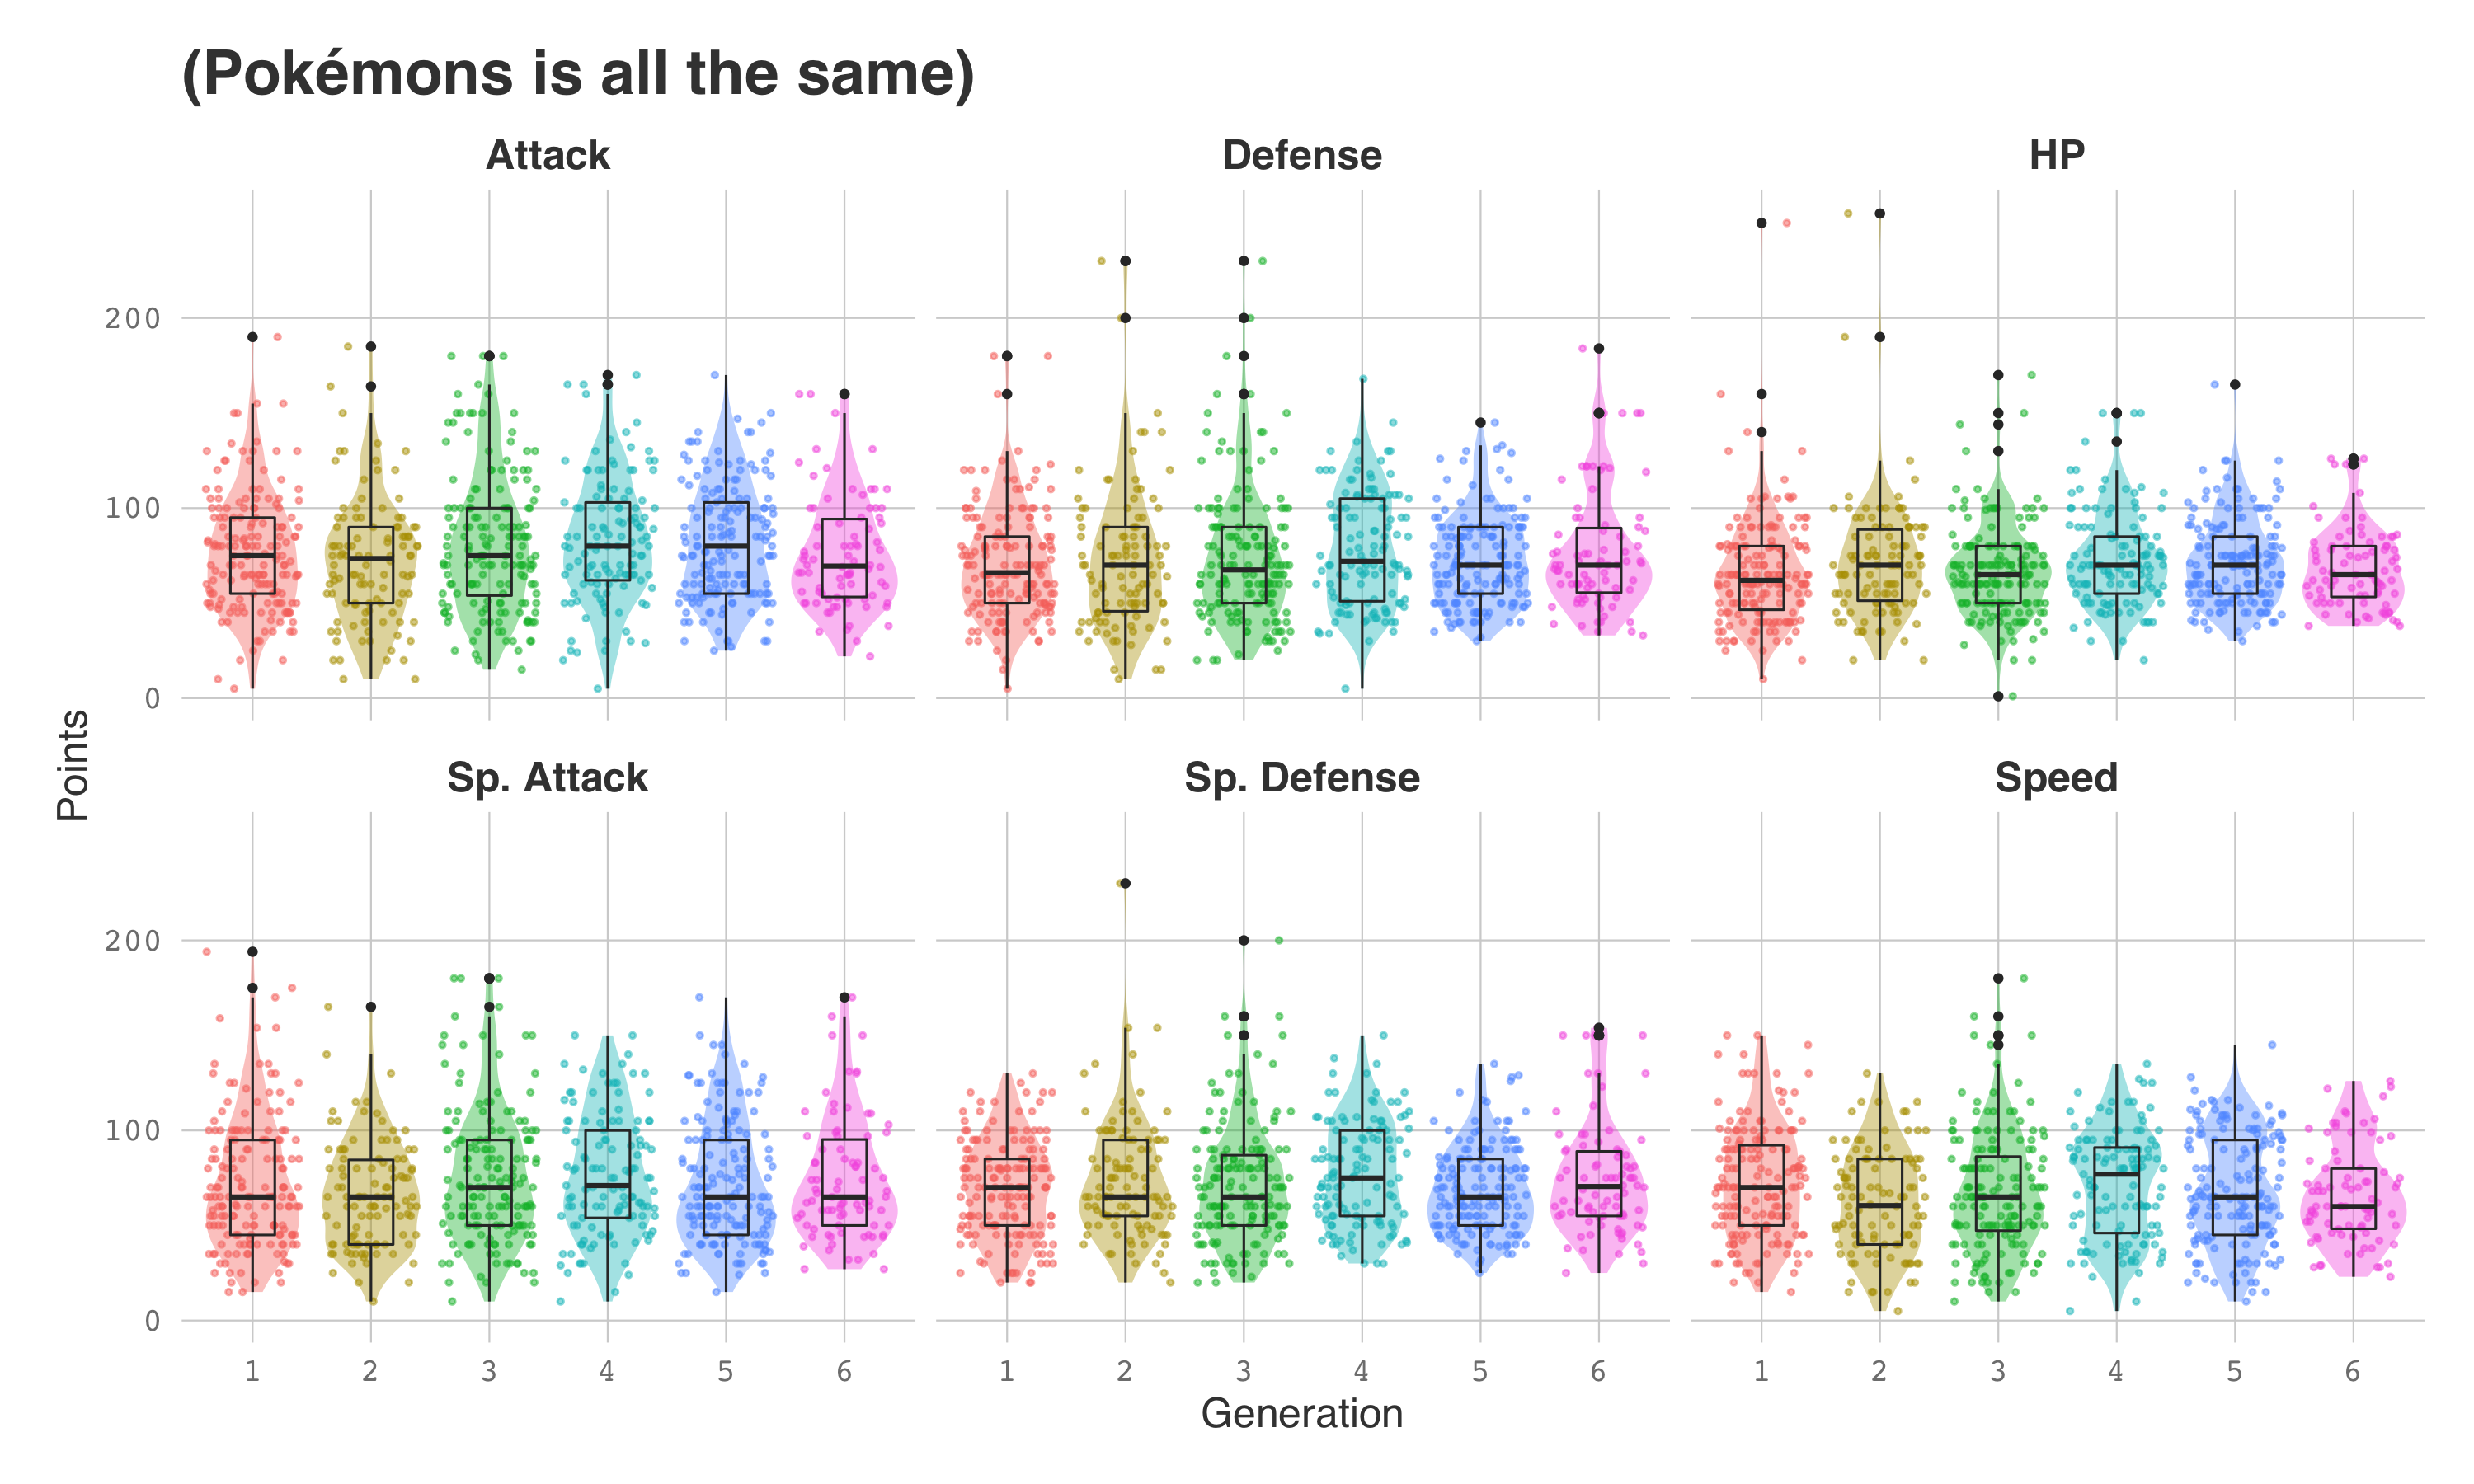
\includegraphics[width = .9\textwidth]{imgs/specs-gen-vio-box.png}
\end{lstlisting}
\end{minipage}
specifies that we want to go into the \lstinline{imgs} folder and include the image called \lstinline{attack-defense.pdf}. We specify the width to be 90 percent of the width of the text block, but we could have specified a width in inches or centimeters. The height is scaled automatically with the width.

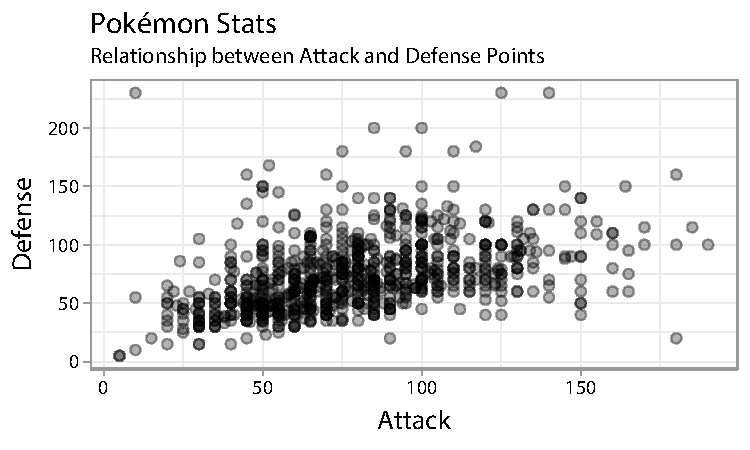
\includegraphics[width = .7\textwidth]{imgs/attack-defense.pdf}


\subsection{Floats}

One great feature of {\LaTeX} is that figures can be allowed to ``float'' to an appropriate position in the text. This lets you write in the code that a figure should go approximately in some place, but the exact position is determined by {\LaTeX}. We recommend the \lstinline{float} package for enhanced float capabilities.

Place a figure in a floating environment using the \lstinline{figure} environment. Floats also allow you to specify captions and labels. If we put the above image into a float, we can add more information about the figure:

\begin{minipage}{\linewidth}
\begin{lstlisting}
  \begin{figure}[ht]
  \centering
  \caption{Distribution of Pok\'emon Stats}
  \label{fig:poke-stats}
  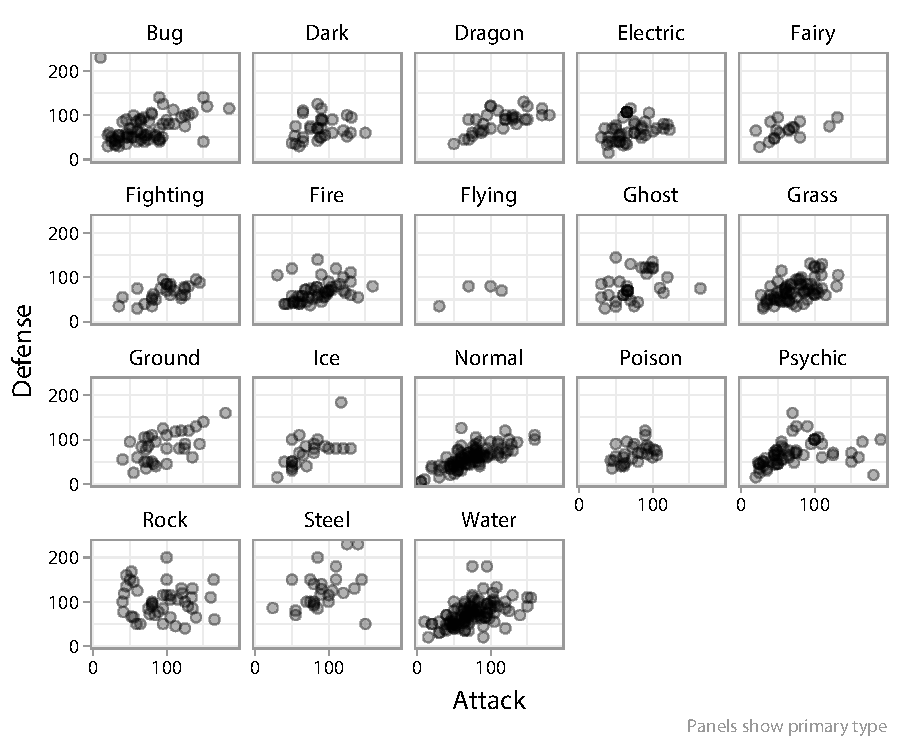
\includegraphics[width = \textwidth]{imgs/attack-defense-type}
  Data source: \url{https://www.kaggle.com/rounakbanik/pokemon}
\end{figure}
\end{lstlisting}
\end{minipage}

\begin{figure}[ht]
  \centering
  \caption{Distribution of Pok\'emon Stats}
  \label{fig:poke-stats}
  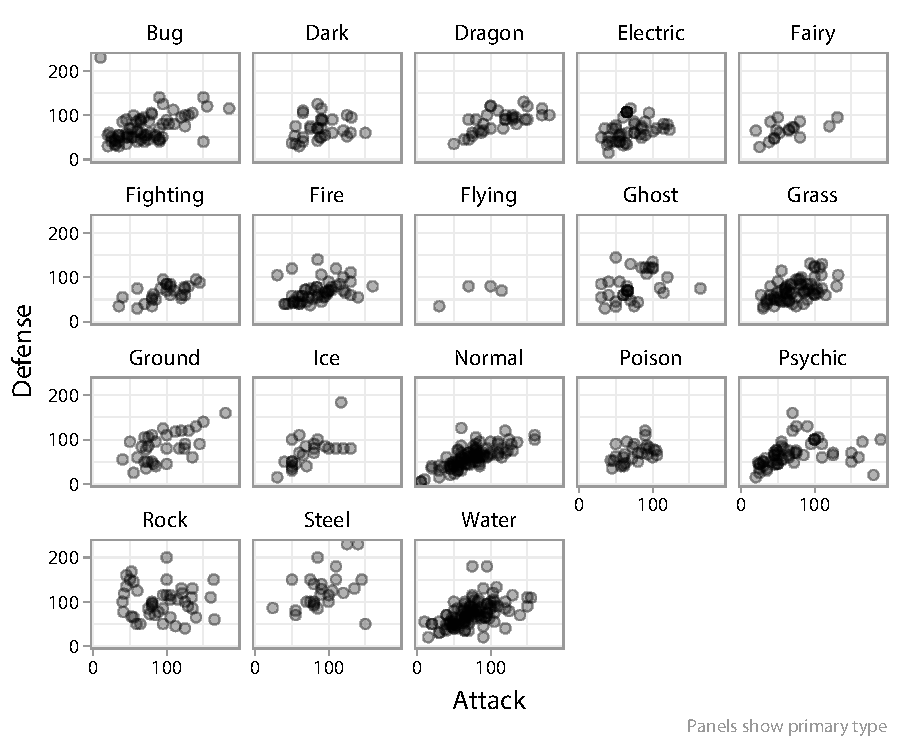
\includegraphics[width = 0.9\textwidth]{imgs/attack-defense-type}
  Data source: \url{https://www.kaggle.com/rounakbanik/pokemon}
\end{figure}



A few other bits of syntax and notes:
\begin{itemize}
  \item \lstinline+[ht]+ locates the float `here' on the page or, if `here' doesn't work, then on the top of the next page. Alternately, can use \lstinline+[t!]+ (`top') or \lstinline+[b!]+ (`bottom'). The exclamation point overrides LaTeX's normal rules for placing figures.
  \item \lstinline+\caption+ inserts a caption. You can use \lstinline+\caption*+ to inset an unnumbered caption.
  \item Several file formats will work, but in general, you should include ``vector'' graphics (such as \texttt{.pdf}s), since they are infinitely scalable without losing image detail. Stata and R can produce \texttt{.pdf} graphics with no problem at all.
\end{itemize}

Labeling floats with the \lstinline+\label{labelname}+ command immediately after the caption allows you automatically to reference the float later using, e.g., \lstinline+Figure~\ref{labelname}+ (the tilde inserts a space that won't break across multiple lines). I could reference Figure~\ref{fig:poke-stats} using \lstinline+Figure~\ref{fig:poke-stats}+. The beauty of {\LaTeX} is that figure number is handled automatically, so you never have to re-number anything if you shuffle the order of figures.%
  \footnote{Try doing that with Microsoft Word!}



\subsubsection{Additional figure capabilities}

Quick things: 

\begin{itemize}
 \item The \lstinline{rotating} package contains the \lstinline{sidewaysfigure} environment, in case you want to rotate a wide figure to fit vertically on the page.
 \item You can place multiple images within the same float, but the float will only have one caption and one label. If you want to have \emph{multiple} captions and multiple labels, however, you can use \lstinline{subcaption} package for the \lstinline{subfloat} environment. 
\end{itemize}




\subsection{Tables}

Tables are created using the \texttt{tabular} environment. Furthermore, place tabulars within the \texttt{table} floating environment to allow for floating placement, captions, labels, and so on. 

\newpage 
This code produces the table below:

\begin{minipage}{\linewidth}
\begin{lstlisting}
  \begin{table}[!ht]
  \begin{center}
  \caption{Selected Films} \label{tab:film}
  \begin{tabular}{l | c | c |  c | D{.}{.}{4}}
             & Acting & Writing   & Effects  & \multicolumn{1}{c}{Plot} \\
  \hline
  Inception  & good   & okay      & great    & 90.52   \\ \hline
  The Artist & great  & none      & B{\&}W   & 100.0   \\ \hline
  Birdemic   & bad    & atrocious & clip art & 3.1     \\ \hline
  Twilight   & none   & none      & sparkly  & .111    \\
  \end{tabular}
  \end{center}
  \end{table}
\end{lstlisting}
\end{minipage}

\begin{table}[ht]
\begin{center}
\caption{Selected Films} \label{tab:film}
  \begin{tabular}{l | c | c |  c | D{.}{.}{4}}
             & Acting & Writing   & Effects  & \multicolumn{1}{c}{Plot} \\
  \hline
  Inception  & good   & okay      & great    & 90.52        \\ \hline
  The Artist & great  & none      & B{\&}W   & 100.0         \\ \hline
  Birdemic   & bad    & atrocious & clip art & 3.1     \\ \hline
  Twilight   & none   & none      & sparkly  & .111    \\
\end{tabular}
\end{center}
\end{table}

What the syntax elements are doing:
\begin{itemize}
  \item The \lstinline+table+ environment is what floats in your document. This environment contains a \lstinline+tabular+ environment that is centered horizontally on the page by the \lstinline+center+ environment.
  \item We've given the table a \lstinline+caption+ and a \lstinline+label+ for referencing Table~\ref{tab:film} in the text. 
  \item \lstinline+{l|c|c...}+ specifies the number of columns, their alignment (\lstinline+c+ = center, \lstinline+l+ = left, \lstinline+r+ = right), and vertical lines ( \lstinline+|+ ) between them.
  %Note the difference between the lower case l- indicating left align, and the | symbol- indicating a vertical line and, typed with shift-backslash.
  \item \lstinline+D{.}{.}{4}+ aligns cells in that column on the decimal point (requires the \texttt{dcolumn} package, see documentation for details).
  \item Cells in the same row are divided by \lstinline+&+ symbols. 
  \item \lstinline+\\+ creates a line break at the end of each row in the table.
  \item \lstinline+\hline+ inserts a horizontal line.
\end{itemize}

Additional notes:
\begin{itemize}
  \item Most textual and mathematical style commands (bold, emphasis, equations, etc.) work within tables.
  \item It's usually best practice to align text to the left, numbers to the right (or numbers with \lstinline+dcolumn+)
  \item Sometimes people mess with the text size in a table if it needs to fit a lot of information. Use with caution. 
  \item Tables can look quite ugly in your source code. Sometimes it can be helpful to turn text wrapping OFF in your text editor to view them more cleanly. Or, you could use careful indentation to keep the code organized.
\end{itemize}


View the source code to examine the following table about detectives.

\begin{table}[!ht]
\begin{center}
\caption{Detective Comparison}\label{det}
\begin{tabular} {l |c c | c c | c c |}
  \multicolumn{1}{c}{} & \multicolumn{2}{c}{L\&O: SVU} & \multicolumn{2}{c}{Literature}  & \multicolumn{2}{c}{Other} \\  \cline{2-7}
                    & Benson     & Stabler  & Holmes & Hardy Boys & Dick Tracy & Batman       \\ \cline{2-7}
  Loose Cannon    & 6       & 10         & 9      & 0        & 3     & 11             \\ \cline{2-7}
  Det. Ability           &  8   & 5     & 10    & 3          & 4      & 11           \\ \cline{2-7}
  Effectiveness   & 80\%  & 70\% & 95\% & 100\%      & 40\%     & 5\% \\ \cline{2-7}
  Tenure (yrs)  & 14+         & 12       & 23        & 1       & 66      & 75              \\ \cline{2-7}
\end{tabular}
\end{center}
\end{table}

Some new syntax introduced:
\begin{itemize}
  \item \lstinline+\cline{2-7}+ inserts horizontal lines across columns 2 through 7.
  \item \lstinline+\multicolumn{2}{c}{text}+ merges adjacent cells to have a multiple-column cell, in this case spanning 2 columns and with center alignment.
\end{itemize}

\subsubsection{Booktabs} 

There exists a table package called \lstinline+booktabs+ that is widely regarded to be \emph{the} way to make prettier tables in {\LaTeX}. The package is designed to facilitate a handful of stylistic improvements on the typical {\LaTeX} table, but with an interface that feels similar. See the documentation for more details.%
  \footnote{\url{http://mirrors.ibiblio.org/CTAN/macros/latex/contrib/booktabs/booktabs.pdf}}
The basic idea is that the table should include:
\begin{itemize}[noitemsep]
  \item More spacious horizontal rules (no double rules)
  \item No vertical rules
\end{itemize}

Compare the following table created using ordinary {\LaTeX} and then \lstinline+booktabs+. (Consult source file for code.)

\begin{table}[H]
\begin{center}
\caption{``Suck It, Trebek'' Trivia Team Details (``vanilla'' {\LaTeX} table)}
\label{tab:booktabs-table}
\begin{tabular}{lrl}
  \hline
  Name        & Year & Topic Strength \\
  \hline
  Richard     & NA   & Comics, Wresting \\
  Jos\'e Luis & 7    & Comics, TV, Movies \\
  Mike        & 5    & NA \\
  Micah       & 5    & American History \\
  Erin        & 4    & Science, Sports \\
  Jordan      & 4    & British History \\
  Rachel      & 6    & Sports, Music \\
  \hline
\end{tabular}
\end{center}
\end{table}


\begin{table}[H]
\begin{center}
\caption{``Suck It, Trebek'' Trivia Team Details (\lstinline+booktabs+ table)}
\label{tab:latex-table}
\begin{tabular}{lrl}
  \toprule
  Name        & Year & Topic Strength \\
  \midrule
  Richard     & NA   & Comics, Wresting \\
  Jos\'e Luis & 7    & Comics, TV, Movies \\
  Mike        & 5    & NA \\
  Micah       & 5    & American History \\
  Erin        & 4    & Science, Sports \\
  Jordan      & 4    & British History \\
  Rachel      & 6    & Sports, Music \\
  \bottomrule
\end{tabular}
\end{center}
\end{table}

Notice how the \lstinline+booktabs+ table just looks, feels, smells better. 

In the code, the main differences you will encounter are the use of \lstinline+\toprule+, \lstinline+\midrule+, and \lstinline+\bottomrule+ (instead of \lstinline+\hline+), and (should you need it) the use of \lstinline+\cmidrule+ instead of \lstinline+\cline+. See documentation for more details.



\subsubsection{Other table advice}

You can create sideways tables with the appropriately named \texttt{sidewaystable} package.


\textbf{Avoid creating tables yourself}. Statistical software contain tools for creating tables in {\LaTeX} code. Hand-typing tables, while \emph{possible}, is prone to error and makes your workflow less reproducible. Creating tables algorithmically is a much better practice. Packages for {\LaTeX} tables include \lstinline{texreg}, \lstinline{xtable}, and \lstinline{stargazer} for R; \lstinline{outtex} for Stata. My choices among R packages are \lstinline+xtable+ for summary statistics and marginals, \lstinline+texreg+ for regression tables.

And \textbf{use booktabs}. It just looks way better.



\section{Math}

One of the most attractive and powerful features of {\LaTeX} is its ability to typeset complex mathematical notation via ``math mode.'' Math mode can be invoked inline by wrapping an expression in dollar signs (\$). For example, \lstinline+$e=mc^2$+, is rendered as $e=mc^2$. Alternatively, a variety of commands allow you set equations apart from the main body of your text. For example:

\begin{minipage}{\linewidth}
\begin{lstlisting}
  \begin{equation}
    y = \alpha + \beta x
  \end{equation}    
\end{lstlisting}
\end{minipage}

Renders as: 
\begin{equation}
  y = \alpha + \beta x
\end{equation}

If you would like to suppress the equation numbering, you can add an asterisk to the end of the command (\lstinline+\begin{equation*}...\end{equation*}+). One nice shorthand: \lstinline+\[...\]+ is equivalent to \lstinline+\begin{equation*}...\end{equation*}+.

Note: equations can be labeled like figures and tables. We could refer to Equation~\ref{eq:mtx-reg} like so:

\begin{equation} \label{eq:mtx-reg}
  y_{i} = X_{i}\beta + \varepsilon_{i}
\end{equation}   

\begin{minipage}{\linewidth}
\begin{lstlisting}
  We could refer to Equation~\ref{eq:mtx-reg} like so:

  \begin{equation} \label{eq:mtx-reg}
    y_{i} = X_{i}\beta + \varepsilon_{i}
  \end{equation}   
\end{lstlisting}
\end{minipage}




\subsection{Fractions}
  
To write fractions, simply use \lstinline+\frac{}{}+ and place the numerator of the fraction in the first set of brackets and the denominator of the fraction in the second set of brackets. For example, $\frac{1}{2}$ or $\frac{1}{n} \sum x_{i}$.

\begin{minipage}{\linewidth}
\begin{lstlisting}
  For example, $\frac{1}{2}$ or $\frac{1}{n} \sum x_{i}$.
\end{lstlisting}
\end{minipage}

It is possible to embed fractions within fractions. 


\subsection{Greek}
  
To write Greek letters, simply write a backslash and the name of the letter after the slash. For example, \lstinline+$\beta$+ and \lstinline+$\sigma$+ renders as $\beta$ and $\sigma$. Capitalizing the first letter of the Greek letter name gives you a capital Greek letter. So, \lstinline+$\Delta$+ renders as $\Delta$, but \lstinline+\delta+ is $\delta$. For some Greek letters, such alpha, the Greek symbol is the same as the Roman symbol. In cases like these, you just use the Roman---there is no \lstinline+$\Alpha$+, only \lstinline+A+.

When there are multiple versions of the same Greek letter, you can use the \lstinline+var+ prefix to use the alternate. For example, \lstinline+$\epsilon = \varepsilon$+ will render as $\epsilon = \varepsilon$. 

A complete list of commands for the Greek alphabet is available at \url{http://jblevins.org/notes/greek}.

\subsection{Operators and Other Symbols}

Numerous symbols can be used in the math environment. Commonly used symbols include inequalities, set notation, and operators. Many of these are straight forward (e.g. equals, greater than, less than), but many are not. We review a few commonly used symbols and operators below. 

To write a summation sign or a product sign, the commands are \lstinline+\sum and \prod+, which produce $\sum$ and $\prod$ respectively. 

For inequalities, the commands are \lstinline+\neq+, \lstinline+\ge+, \lstinline+\le+, and these produce $\neq$, $\ge$, and $\le$ respectively. 

Common set notation commands include \lstinline+\mathbb{R}+ ($\mathbb{R}$), \lstinline+\in+ ($\in$), \lstinline+\not \in+ ($\not \in$), \lstinline+\mid+ ($\mid$). Because curly braces are interpreted by the {\LaTeX} compiler, you need to escape them with a backslash whenever you use them in math mode---you must write \lstinline+\{...\}+ to get $\{...\}$. Putting it all together, we can write \lstinline+$\mathbb{A} \in \{1,2,3\}$+, which will render as $\mathbb{A} \in \{1,2,3\}$.

You may also want to be aware that operators and functions like $\max(x)$, $\ln(x)$, $\lim\limits_{x \to \infty}$, $\int$, and $\partial$ are also {\LaTeX} commands. You can read more about these and other commands here: \url{http://en.wikibooks.org/wiki/LaTeX/Mathematics}.


\subsection{Hats and Bars}

To place a hat or a bar over any math character, simply place the text in brackets after the writing \lstinline+\bar{}+ or \lstinline+\hat{}+ commands. \lstinline+$\bar{\beta} \neq \hat{y}$+ gives us $\bar{\beta} \neq \hat{y}$.


\subsection{Superscripts and Subscripts}

To write a superscript, write \lstinline+^{}+ with the text of the superscript in the brackets. If you just have one character in the superscript, you do not have to include the brackets. For example, \lstinline+$x^3$+ renders as $x^3$ or \lstinline+$e^{-z\gamma}$+ renders as $e^{-z\gamma}$. If you want to put multiple characters into the superscript but forget the brackets (\lstinline+$e^-z\gamma$+), only the first character will be in the superscript ($e^-z\gamma$). 

To write a subscript, write \lstinline+_{}+ with the text of the subscript in the brackets. Again, if you have just one character in the subscript, you do not have to include the brackets. For example, \lstinline+$x_1$+ renders as $x_1$ and \lstinline+$x_{ij}$+ renders as $x_{ij}$. 

Some commands allow you to use the subscript and superscript environments together to place notation on top of or underneath other notation. For example, \lstinline+$\sum_{i=0}^{100} i$+ renders as $\sum_{i=0}^{100} i$. To make these commands look a little better, we can add the command \lstinline+\limits+ after the \lstinline+\sum+ command: \lstinline+$\sum\limits_{i=0}^{100} i$+. From this we get: $\sum\limits_{i=0}^{100} i$. We can also accomplish this by including \lstinline+\displaystyle+ before the expression: \lstinline+\displaystyle \sum_{i=0}^{100} i+ gives us $\displaystyle \sum_{i=0}^{100} i$. This can also improve limit expressions ($\displaystyle\lim_{x\to\infty}$) and integrals ($\displaystyle\int^y_x$). Display style will also slightly increase the size of your expressions in in-line math, which can prevent complicated math from getting shrunk too small in the middle of a block of text.


\subsection{Multiple, aligned equations}

To align multiple equations together, you can use the \lstinline{align} environment, which will align a set of equations along an operator of your choice. To pick the operator on which you want to align your list of equations, place a \lstinline+&+ in front of it. For multiple lines, you need to place two backslashes at the end of each line of equations, and there should be no empty lines anywhere in the \lstinline+align+ environment. 

The following code\ldots \\
\begin{minipage}{\linewidth}
\begin{lstlisting}
  \begin{align}
    \ln(L) &= n \ln(\alpha) + n \ln (x) - n \ln (x) \\
    \frac{d \ln(L)}{d\alpha} &= \frac{n}{\alpha} + n \ln(x) - 0 \\
    \frac{n}{\alpha} + n \ln(x) &= 0 \\
    \frac{n}{\alpha} &= -n \ln(x) \\
    n &= \alpha (-n \ln(x)) \\
    \alpha &= \frac{n}{-n \ln(x)} \\
    \alpha &= \frac{-1}{\ln(x)}
  \end{align}
\end{lstlisting}
\end{minipage}
\ldots will render as\ldots
\begin{align}
  \ln(L) &= n \ln(\alpha) + n \ln (x) - n \ln (x)\\
  \frac{d \ln(L)}{d\alpha} &= \frac{n}{\alpha} + n \ln(x) - 0\\
  \frac{n}{\alpha} + n \ln(x) &= 0\\
  \frac{n}{\alpha} &= -n \ln(x)\\
  n &= \alpha (-n \ln(x))\\
  \alpha &= \frac{n}{-n \ln(x)}\\
  \alpha &= \frac{-1}{\ln(x)}\\
\end{align}

You can suppress equation numbering, again, by typing \lstinline{align*} (with an asterisk) instead of \lstinline{align}.

Split a numbered equation across multiple lines using the \lstinline{split} environment within \lstinline{align}:

\begin{align}
  \begin{split}
    y_{i} &= \hat{y}_{i} + \varepsilon_{i} \\
    y_{i} &= \hat{\alpha} + \hat{\beta}x_{i} + \varepsilon_{i}
  \end{split}
\end{align}

The \lstinline{align} environment is useful enough to replace the \lstinline{equation} environment, in my opinion.

If your equations are getting too smushed together, you can add additional space (or subtract space) between lines by specifying skip lengths in square brackets. Example: \\
\begin{minipage}{\linewidth}
\begin{lstlisting}
  \begin{align*}
    a &= 1 \\
    a &= 1 \\[6pt]
    a &= 1 \\[12pt]
    a &= 1
  \end{align*} 
\end{lstlisting}
\end{minipage}
\.dots renders as\ldots
\begin{align*}
  a &= 1 \\
  a &= 1 \\[6pt]
  a &= 1 \\[12pt]
  a &= 1
\end{align*}


\subsection{Flexible brackets}

Sometimes the stuff you want to put inside of parentheses is bigger than the parentheses themselves. For example:
\begin{align*}
 (\frac{1}{n})
\end{align*}

You can create size-flexible brackets by prefacing the bracket symbols with \lstinline+\left+ and \lstinline+\right+. If you type \lstinline+\left( \frac{1}{n} \right)+:
\begin{align*}
 \left( \frac{1}{n} \right)
\end{align*}

This trick works with parens, square brackets, curly brackets, etc.






\subsection{Arrays and Matrices}

Tables, meet math. If you want to create a table in math mode, you can use the \lstinline+array+ environment, which behaves basically like the \lstinline+tabular+ environment. They are useful for piecewise functions:

\begin{minipage}{\linewidth}
\begin{lstlisting}
  \begin{align*}
    f(x) &= \left\{ 
              \begin{array}{ll}
                -x & \text{ if $x < 0$} \\ 
                1 & \text{ if $x = 0$} \\ 
                x^{2} & \text{ if $x > 0$} \\ 
              \end{array} 
            \right.
  \end{align*}
\end{lstlisting}
\end{minipage}

\begin{align*}
  f(x) &= \left\{ 
            \begin{array}{ll}
              -x & \text{ if $x < 0$} \\ 
              1 & \text{ if $x = 0$} \\ 
              x^{2} & \text{ if $x > 0$} \\ 
            \end{array} 
          \right.
\end{align*}

There are also matrix environments for math mode (with the \lstinline+amsmath+ package), which place a table inside of various kinds of brackets. I tend to use \lstinline+bmatrix+ for square bracket matrices.

\begin{minipage}{\linewidth}
\begin{lstlisting}
  \begin{align*}
    \begin{bmatrix}
      4 & 5  \\
      2 & 0  \\
      1 & 7
    \end{bmatrix}
    \times
    \begin{bmatrix}
      8 & 4 & 0  \\
      6 & 3 & 4
    \end{bmatrix}
    &=
    \begin{bmatrix}
      62 & 31 & 20  \\
      16 & 8  & 0  \\
      50 & 25 & 28 
    \end{bmatrix}
  \end{align*}
\end{lstlisting}
\end{minipage}
\begin{align*}
  \begin{bmatrix}
    4 & 5  \\
    2 & 0  \\
    1 & 7
  \end{bmatrix}
  \times
  \begin{bmatrix}
    8 & 4 & 0  \\
    6 & 3 & 4
  \end{bmatrix}
  &=
  \begin{bmatrix}
    62 & 31 & 20  \\
    16 & 8  & 0  \\
    50 & 25 & 28 
  \end{bmatrix}
\end{align*}


You can also use various \lstinline+\dots+ commands for matrices, like with this monstrosity:
\begin{align*}
  \begin{bmatrix}
    1      & 0 & \cdots & 0      \\
    0      & 1 &        & \vdots \\
    \vdots &   & \ddots & 0      \\
    0 & \cdots &      0 & 1 
  \end{bmatrix}
\end{align*}



\newpage

\section{Good {\LaTeX} Practices}

\begin{itemize}
  \item \textbf{Minimize stylistics interventions}. {\LaTeX} is built on a philosophy that you should be concerned with the content of the document, not be preoccupied with controlling the stylistic details. Try not to overly style your documents. If you want to intervene, it's always better to intervene with global settings (in the preamble), since they can be easily modified later and universally applied through the document.
  \item \textbf{Take content control seriously.} {\LaTeX} can be integrated into the social science workflow in a number of ways. To minimize human error (and save time and effort), export figures and tables directly from Stata or R and then import them with {\LaTeX}. You can also do this with statistics such as $p$-values so that your document is always up-to-date with your most recent analysis!
  \item \textbf{Re-use code}. Copy and paste from old code you or someone else created, and modify as needed. No need to reinvent the wheel every time. Make a blank \texttt{.tex} file that has a preamble using your most-used external packages, keep it somewhere safe, and start all fresh papers with that template. % This code included.
  \item \textbf{Include comments}. Particularly as you're still learning, it's a good idea to write comments in your code to explain why you're doing things or how you're doing it.  It's also a nice way to include content that you're not sure if you'll use---put it in a comment and you still have it later if you want it back in.
  \item \textbf{Whenever you open a bracket or an environment, close it immediately}. Whether you're beginning and ending environments or opening and closing parenthesis or brackets, always put the end in right away, then fill in the content in between. This will greatly cut down on syntax errors from forgetting to close things once you've gotten distracted by the substance. Some software will do this for you, so find handy software!
  \item \textbf{Compile early and often}. Bugs can be hard to find, so if you write a long document and it won't compile it is often frustrating and time-consuming to figure out where it's getting tripped up.  Compile often---anytime you do anything new or complicated---to make sure it's working; that way when errors occur you'll know where they are.
  \item \textbf{Debug in the order the errors appear.} When debugging a {\LaTeX} document, make sure that you start by fixing errors as early in the document as you can. Errors tend to cascade---failing to close an environment early in the document can result in multiple other problems later in the document. 
  \item \textbf{Comment-out lines to debug}. If you're getting errors and can't figure out why, try commenting-out complicated parts here and there to find the source that's tripping it up.
\end{itemize}


\section{Useful Resources}

\begin{itemize}
  \item The Comprehensive \TeX~Archive Network (\url{http://www.ctan.org}).  In particular see the `Not So Short' guide at \url{http://ctan.tug.org/tex-archive/info/lshort/english/lshort.pdf} with tons of information on beginning and advanced topics.
  \item The {\LaTeX} Wikibook (\url{https://en.wikibooks.org/wiki/LaTeX}). This is how I (Michael DeCrescenzo) learned {\LaTeX}.
  \item {\TeX} Exchange (\url{http://tex.stackexchange.com/}). This site collects user questions related to working with {\LaTeX}. Other users offer answers and can ``upvote'' the best answers. The large user base results in very high quality answers to both common and obscure questions. Don't be afraid to post a question if you're unable to figure out a given issue. 
  \item Crash Course in {\LaTeX} (\url{http://haptonstahl.org/latex/}). A very nice user-friendly website guide to {\LaTeX}, created by a Steve Haptonstahl, a (former) political methodologist.
  \item Google (\url{https://www.google.com/}). If all else fails (or, perhaps, before searching through pages and pages of documentation) just search for what you're looking for --- there will be a user group discussion or a guide posted somewhere that explains how to do it.
  \item Wikipedia's List of {\LaTeX} editors (\url{http://en.wikipedia.org/wiki/Comparison_of_TeX_editors}). There are various alternative {\LaTeX} editors that are of varying degrees of quality and price. Many are better than the default editors that come with various TeX distributions.  
  \item Detexify (\url{http://detexify.kirelabs.org}). Need to include a symbol but don't know what it's called or how to enter it into LaTex? Draw the symbol using this tool, and the program will return the command to draw it. For example, draw that ``trident-looking thing'' and the tool will tell you how to make a $\psi$.
  \item Overleaf (\url{https://www.overleaf.com/}). Cloud-based {\LaTeX} editor which allows documents to be edited by multiple individuals at the same time and which compiles in real-time. 
\end{itemize}



\end{document}